\section{ITU-MiniTwit}
Our MiniTwit is an 'X' (formerly known as Twitter) clone written in golang. It is a project which continues development on the ITU-MiniTwit system presented in the course DevOps, and it consists of a web service, as well as an API service. 

\subsection{Architecture of MiniTwit}
MiniTwit follows the server-client architecture, and the server is deployed via a Docker Swarm, which consists of virtual machines (aka 'droplets') on DigitalOcean. Data, such as user-data, messages and followers are stored in a PostgreSQL database, which is also hosted on DigitalOcean. \\
In the swarm, we have manager-nodes and worker-nodes. The only services allowed to run on the managers are Prometheus and Dozzle (more about the swarm services in section 4). Figure \ref{fig:DeployDiagram} is a Specification Level Deployment Diagram, which shows how ITU-MiniTwit is deployed on a worker-node.
\begin{figure}[h]
\centering
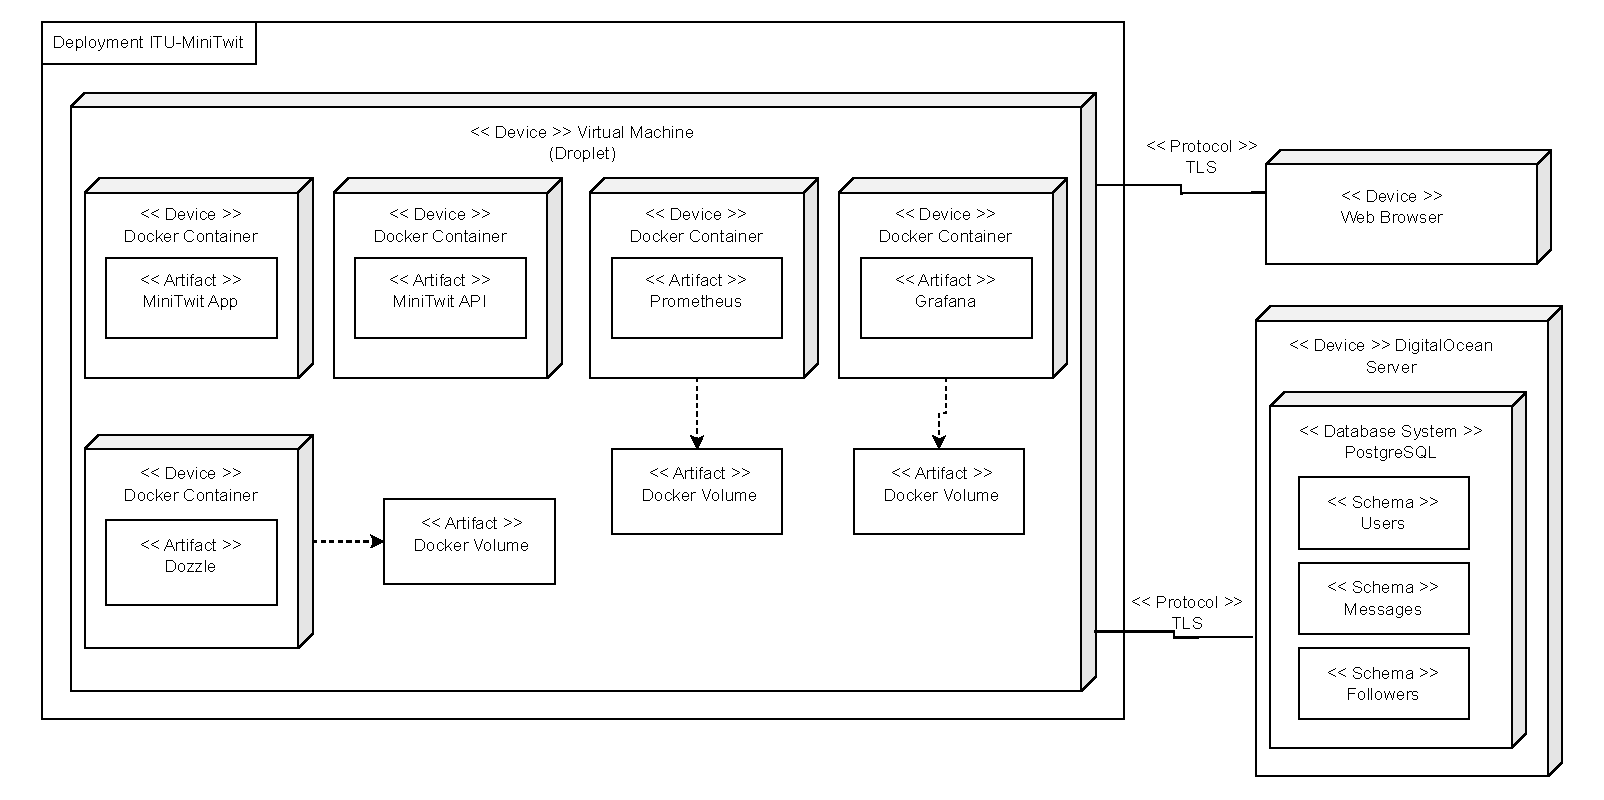
\includegraphics[width=\textwidth]{images/DeployDiagramWIP.pdf}
\caption{WIIIP}
\label{fig:DeployDiagram}
\end{figure}

\subsection{Dependencies of MiniTwit}
--MISSING--
\subsection{System Interactions}
--MISSING--\\
user request + simulator request

\section{Current state of our MiniTwit}
We have implemented the two tools Sonarqube and Code Climate, which can assist in estimating the maintainability and technical debt of our project.
\subsection{Code Climate}
Code Climate reports 10 code smells, 0 duplications and 0 other issues. This leaves us with an A-rank (see figure \ref{fig:CodeClimate})\\
\begin{figure}[h]
\centering
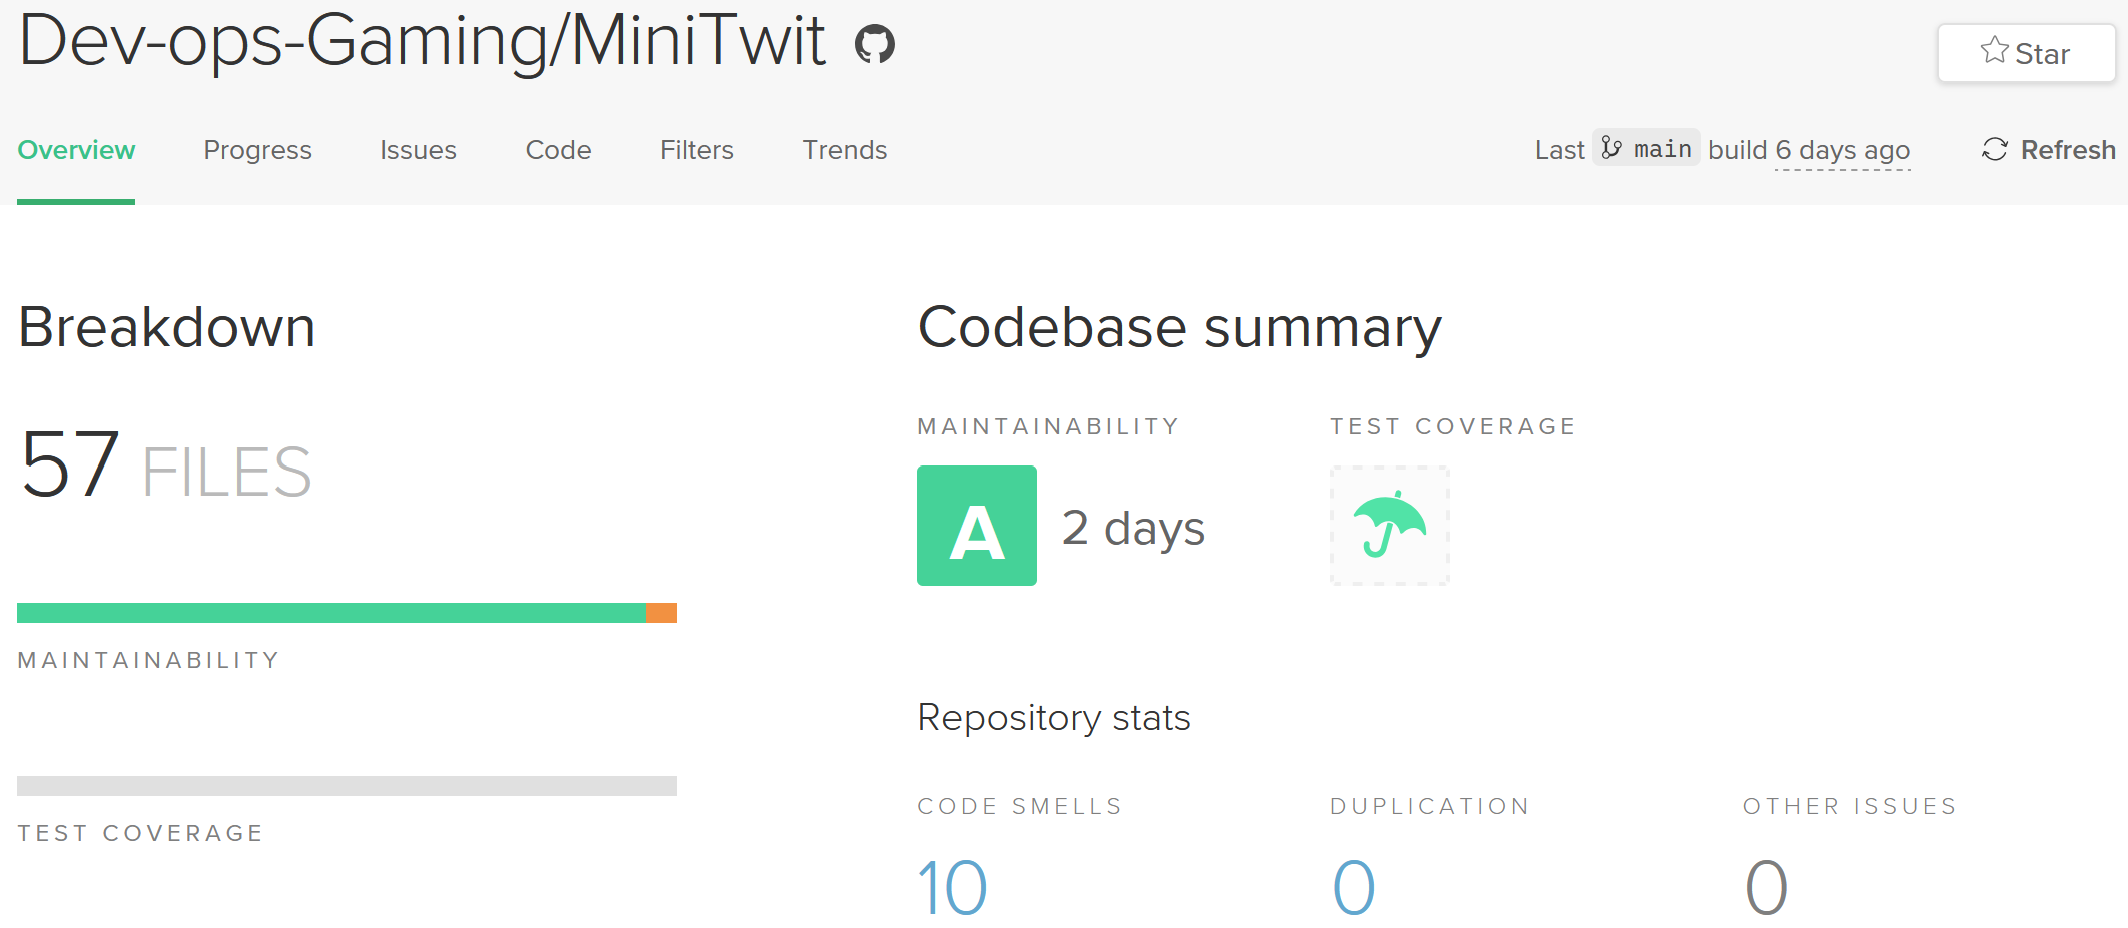
\includegraphics[width=\textwidth]{images/code_climate.png}
\caption{Bitch?}
\label{fig:CodeClimate}
\end{figure}

\subsection{Sonarqube}
Sonarqube reports 18 issues - all in the category 'maintainability' - and 0.9\% code duplication (see figure \ref{fig:SonarQube}). A majority of these issues are found in the tests, and many of the issues are in regards to string duplicates.
\begin{figure}[h]
\centering
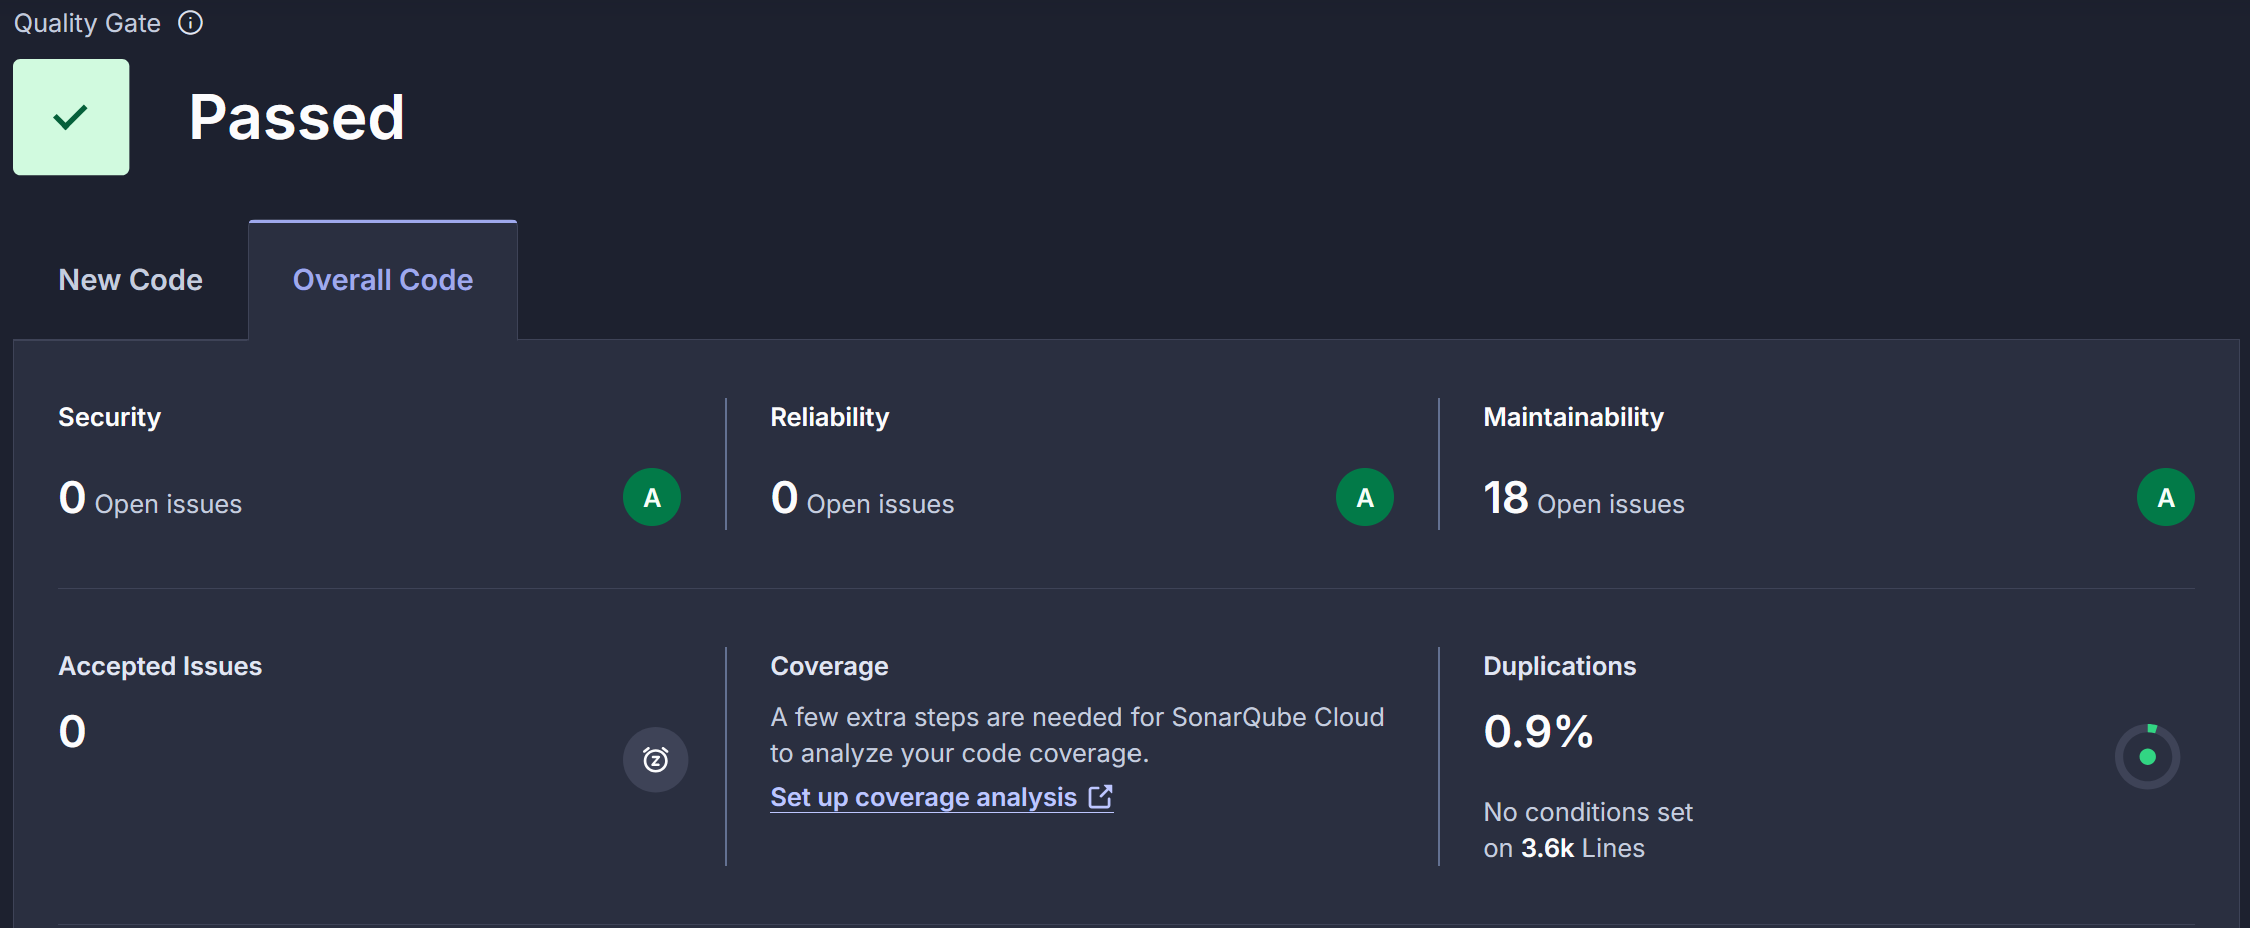
\includegraphics[width=\textwidth]{images/sonarQube.png}
\caption{We need to fix position of this wehn report almost done}
\label{fig:SonarQube}
\end{figure}
